\documentclass[conference]{IEEEtran}
\usepackage[utf8]{inputenc}
\usepackage[T1]{fontenc}
\usepackage{cite}
\usepackage{amsmath,amssymb,amsfonts}
\usepackage{algorithmic}
\usepackage{graphicx}
\usepackage{textcomp}
\usepackage{xcolor}
\usepackage{booktabs}
\usepackage{listings}
\usepackage{subcaption}
\usepackage{url}


\usepackage[hidelinks]{hyperref}


\begin{document}

\title{}

\maketitle

\begin{abstract}

\end{abstract}

\section{Introduction}

\section{Methodology}

\subsection{Data Import and Exploration}
\label{sec:data_import_exploration}

\subsubsection{Dataset Overview and Problem Formulation}
The experimental dataset, designated as \texttt{Gold\_data.csv}, captures historical daily trading observations for gold assets. The raw dataset comprises $N = 6{,}399$ observations and $M = 8$ attributes, spanning over two decades of financial records. In accordance with the project objectives, the predictive target variable is formally established as:
\begin{equation}
    y = \text{Close}
\end{equation}
which represents the daily closing price of gold. The remaining seven attributes constitute the initial candidate input feature space:
\begin{equation}
    \mathbf{x} = \left[ \text{Date}, \text{Open}, \text{High}, \text{Low}, \text{Volume}, \text{Sales}, \text{weight} \right]^T
\end{equation}

Table~\ref{tab:dataset_summary} details the statistical properties, data types, missing value counts, and zero occurrences across all attributes prior to any transformation.

\begin{table*}[t]
\caption{Descriptive Statistics and Initial Data Profiling ($N = 6{,}399$)}
\label{tab:dataset_summary}
\centering
\small
\begin{tabular}{lcrrrrrrrrr}
\hline
\textbf{Variable} & \textbf{Role} & \textbf{Type} & \textbf{Missing} & \textbf{Zeros} & \textbf{Mean} & \textbf{Std. Dev.} & \textbf{Min} & \textbf{Median} & \textbf{Max} \\
\hline
\texttt{Date}   & Feature & String  & 0   (0.00\%)  & 0   & ---         & ---        & ---      & ---      & ---        \\
\texttt{Open}   & Feature & Float64 & 0   (0.00\%)  & 0   & 1,274.89    & 782.87     & 255.00   & 1,251.60 & 5,415.70   \\
\texttt{High}   & Feature & Float64 & 0   (0.00\%)  & 0   & 1,281.73    & 788.80     & 256.10   & 1,256.20 & 5,586.20   \\
\texttt{Low}    & Feature & Float64 & 0   (0.00\%)  & 0   & 1,267.91    & 777.09     & 255.00   & 1,244.80 & 5,334.90   \\
\texttt{Close}  & \textbf{Target} & Float64 & 0   (0.00\%)  & 0   & 1,274.96    & 783.12     & 255.10   & 1,251.10 & 5,377.30   \\
\texttt{Volume} & Feature & Int64   & 0   (0.00\%)  & 418 & 4,282.54    & 24,051.64  & 0.00     & 117.00   & 386,334.00 \\
\texttt{Sales}  & Feature & Float64 & 937 (14.64\%) & 0   & 25,302.83   & 14,182.08  & 1,015.41 & 25,123.10& 49,988.50  \\
\texttt{weight} & Feature & Float64 & 0   (0.00\%)  & 0   & 60.62       & 28.87      & 11.66    & 54.67    & 364.23     \\
\hline
\end{tabular}
\end{table*}

\subsubsection{Target Variable Characterization}
Understanding the statistical distribution of the target variable $y = \text{Close}$ is critical for selecting subsequent feature scaling and transformation methods. The distribution exhibits:
\begin{itemize}
    \item \textbf{Central Tendency and Dispersion:} A sample mean of $\mu = 1{,}274.96$ and standard deviation of $\sigma = 783.12$, with an interquartile range (IQR) spanning from $Q_1 = 651.70$ to $Q_3 = 1{,}695.65$.
    \item \textbf{Skewness:} A Fisher-Pearson coefficient of skewness of $\gamma_1 = 1.4181$, indicating a pronounced right-tailed asymmetric distribution driven by historical secular bull market regimes in gold.
    \item \textbf{Kurtosis:} A sample kurtosis of $\gamma_2 = 3.7962$, confirming heavier tails than a normal distribution and the occurrence of significant price extensions.
\end{itemize}

\subsubsection{Data Profiling and Identified Irregularities}
An automated screening of the raw observations revealed four key categories of data quality irregularities that must be systematically addressed during the data cleaning stage:

\begin{enumerate}
    \item \textbf{Missing Values in \texttt{Sales}:} Exactly $937$ observations ($14.64\%$ of the dataset) have missing (\texttt{NaN}) entries in the \texttt{Sales} column. Since neural network architectures cannot process missing values directly, an appropriate imputation strategy (e.g., forward-fill or median interpolation) or feature evaluation is required.
    \item \textbf{Zero-Volume Regimes:} The \texttt{Volume} attribute contains $418$ instances of exact zero values ($6.53\%$). In financial asset pricing, zero daily volume frequently corresponds to non-trading holidays, exchange closures, or reporting latency, which distort liquidity modeling.
    \item \textbf{Logical Price Boundary Inconsistencies:} In classical financial Open-High-Low-Close (OHLC) bar structures, the physical constraints $Low \le \min(Open, Close)$ and $High \ge \max(Open, Close)$ must hold strictly. Our screening identified:
    \begin{itemize}
        \item $1$ observation where $High < Low$.
        \item $430$ observations where $Close \notin [Low, High]$.
    \end{itemize}
    These anomalies point to transcription errors or inverted column mappings in the original source data that require reconciliation.
    \item \textbf{Temporal Representation Heterogeneity:} The \texttt{Date} attribute is currently formatted as a heterogeneous object string, containing $3{,}865$ dates with hyphen delimiters (e.g., \texttt{30-08-00}) and $2{,}534$ dates with slash delimiters (e.g., \texttt{1/9/2000}). Robust two-digit vs.\ four-digit year parsing is necessary to ensure chronological sorting and temporal integrity.
\end{enumerate}

\subsection{Data Cleaning and Preprocessing}
\label{sec:data_cleaning}

Data cleaning constitutes a foundational step to ensure numerical stability and physical validity before statistical modeling. The empirical strategy developed for this stage addresses the four irregularities identified during initial data profiling.

\subsubsection{Temporal Alignment and Formatting}
The \texttt{Date} attribute was parsed using a mixed-format day-first date parser, mapping both hyphenated (\texttt{DD-MM-YY}) and slashed (\texttt{D/M/YYYY}) timestamp strings into standard 64-bit datetime representations (\texttt{datetime64[ns]}). Observations were verified to be monotonically increasing from August 30, 2000, through March 3, 2026 ($N = 6{,}399$), guaranteeing rigorous chronological ordering without forward-looking temporal leaks.

\subsubsection{OHLC Envelope Boundary Reconciliation}
In standard financial time-series recording, price bars must strictly satisfy the geometric and physical boundaries of the trading session:
\begin{align}
    \text{High}_t &\ge \max(\text{Open}_t, \text{Close}_t, \text{Low}_t) \\
    \text{Low}_t  &\le \min(\text{Open}_t, \text{Close}_t, \text{High}_t)
\end{align}

Inspection of the raw dataset revealed $1$ observation where $\text{High} < \text{Low}$ and $430$ observations where $\text{Close} \notin [\text{Low}, \text{High}]$. These anomalies stem from asynchronous settlement recording versus intraday electronic quote tracking. Rather than pruning $6.7\%$ of the dataset, which would induce temporal discontinuities, an envelope reconciliation projection was applied:
\begin{align}
    \text{High}^*_t &= \max(\text{High}_t, \text{Open}_t, \text{Close}_t) \\
    \text{Low}^*_t  &= \min(\text{Low}_t, \text{Open}_t, \text{Close}_t)
\end{align}
This formulation guarantees 100\% mathematical consistency with zero row discards.

\subsubsection{Imputation of Missing Sales}
A total of $937$ missing observations ($14.64\%$) were present in the \texttt{Sales} feature. Given the continuous, sequential nature of financial trading activity, mean or global median imputation would artificially flatten the variance and distort autocorrelation structures. Hence, a forward/backward-bounded piecewise linear time-series interpolation was employed:
\begin{equation}
    \text{Sales}_t = \text{Sales}_{t_a} + (t - t_a) \frac{\text{Sales}_{t_b} - \text{Sales}_{t_a}}{t_b - t_a}
\end{equation}
where $t_a$ and $t_b$ represent the closest preceding and succeeding valid trading days, respectively. This retains smooth sample continuity across the entire 26-year horizon.

\subsubsection{Zero-Volume Rectification}
The \texttt{Volume} variable exhibited $418$ occurrences ($6.53\%$) of exact zeros, predominantly clustered in historical trading years (2000--2005) due to reporting latency on thin trading sessions. Because neural network workflows frequently apply logarithmic compression ($\ln(1 + \text{Volume})$), zero entries create artificial floor boundary artifacts. Zero-volume records were treated as temporary unrecorded liquidity windows and resolved via linear interpolation bounded by adjacent active sessions, raising the global minimum to $\text{Volume}_{\min} = 1$ without altering the heavy-tailed upper quantiles.

\subsubsection{Price Outlier Justification: Secular Trend vs. Spurious Noise}
Evaluating the price attributes ($\text{Close}$, $\text{Open}$, $\text{High}$, $\text{Low}$) under the standard Tukey interquartile range criterion ($Q_3 + 1.5 \times \text{IQR}$) identifies $213$ observations above $\$3{,}261.57$ (up to $\$5{,}377.30$) as statistical outliers. 

\textbf{Methodological Decision:} No clipping, winsorization, or trimming was performed on the price series or the target variable $\text{Close}$. These values correspond to authentic macroeconomic secular appreciation in gold prices observed between 2024 and 2026. Truncating these points would impose an artificial ceiling on the target distribution and severely degrade the predictive fidelity of any downstream neural network. Non-linear scaling will be addressed systematically in the Feature Transformation phase.

\begin{table}[htbp]
\caption{Comparative Data Cleaning Metrics (Before vs. After)}
\label{tab:cleaning_summary}
\centering
\small
\begin{tabular}{lccc}
\toprule
\textbf{Metric} & \textbf{Raw Data} & \textbf{Cleaned Data}  \\
\midrule
Total Observations ($N$)   & 6,399          & 6,399     \\
Missing \texttt{Sales}    & 937 (14.64\%)  & 0 (0.00\%)      \\
Zero \texttt{Volume}      & 418 (6.53\%)   & 0 (0.00\%)      \\
$\text{High} < \text{Low}$ & 1 & 0      \\
$\text{Close} \notin [\text{Low}, \text{High}]$ & 430 & 0     \\
Temporal Format           & Mixed strings  & \texttt{datetime64[ns]} \\
\bottomrule
\end{tabular}
\end{table}

\begin{figure}[htbp]
\centering
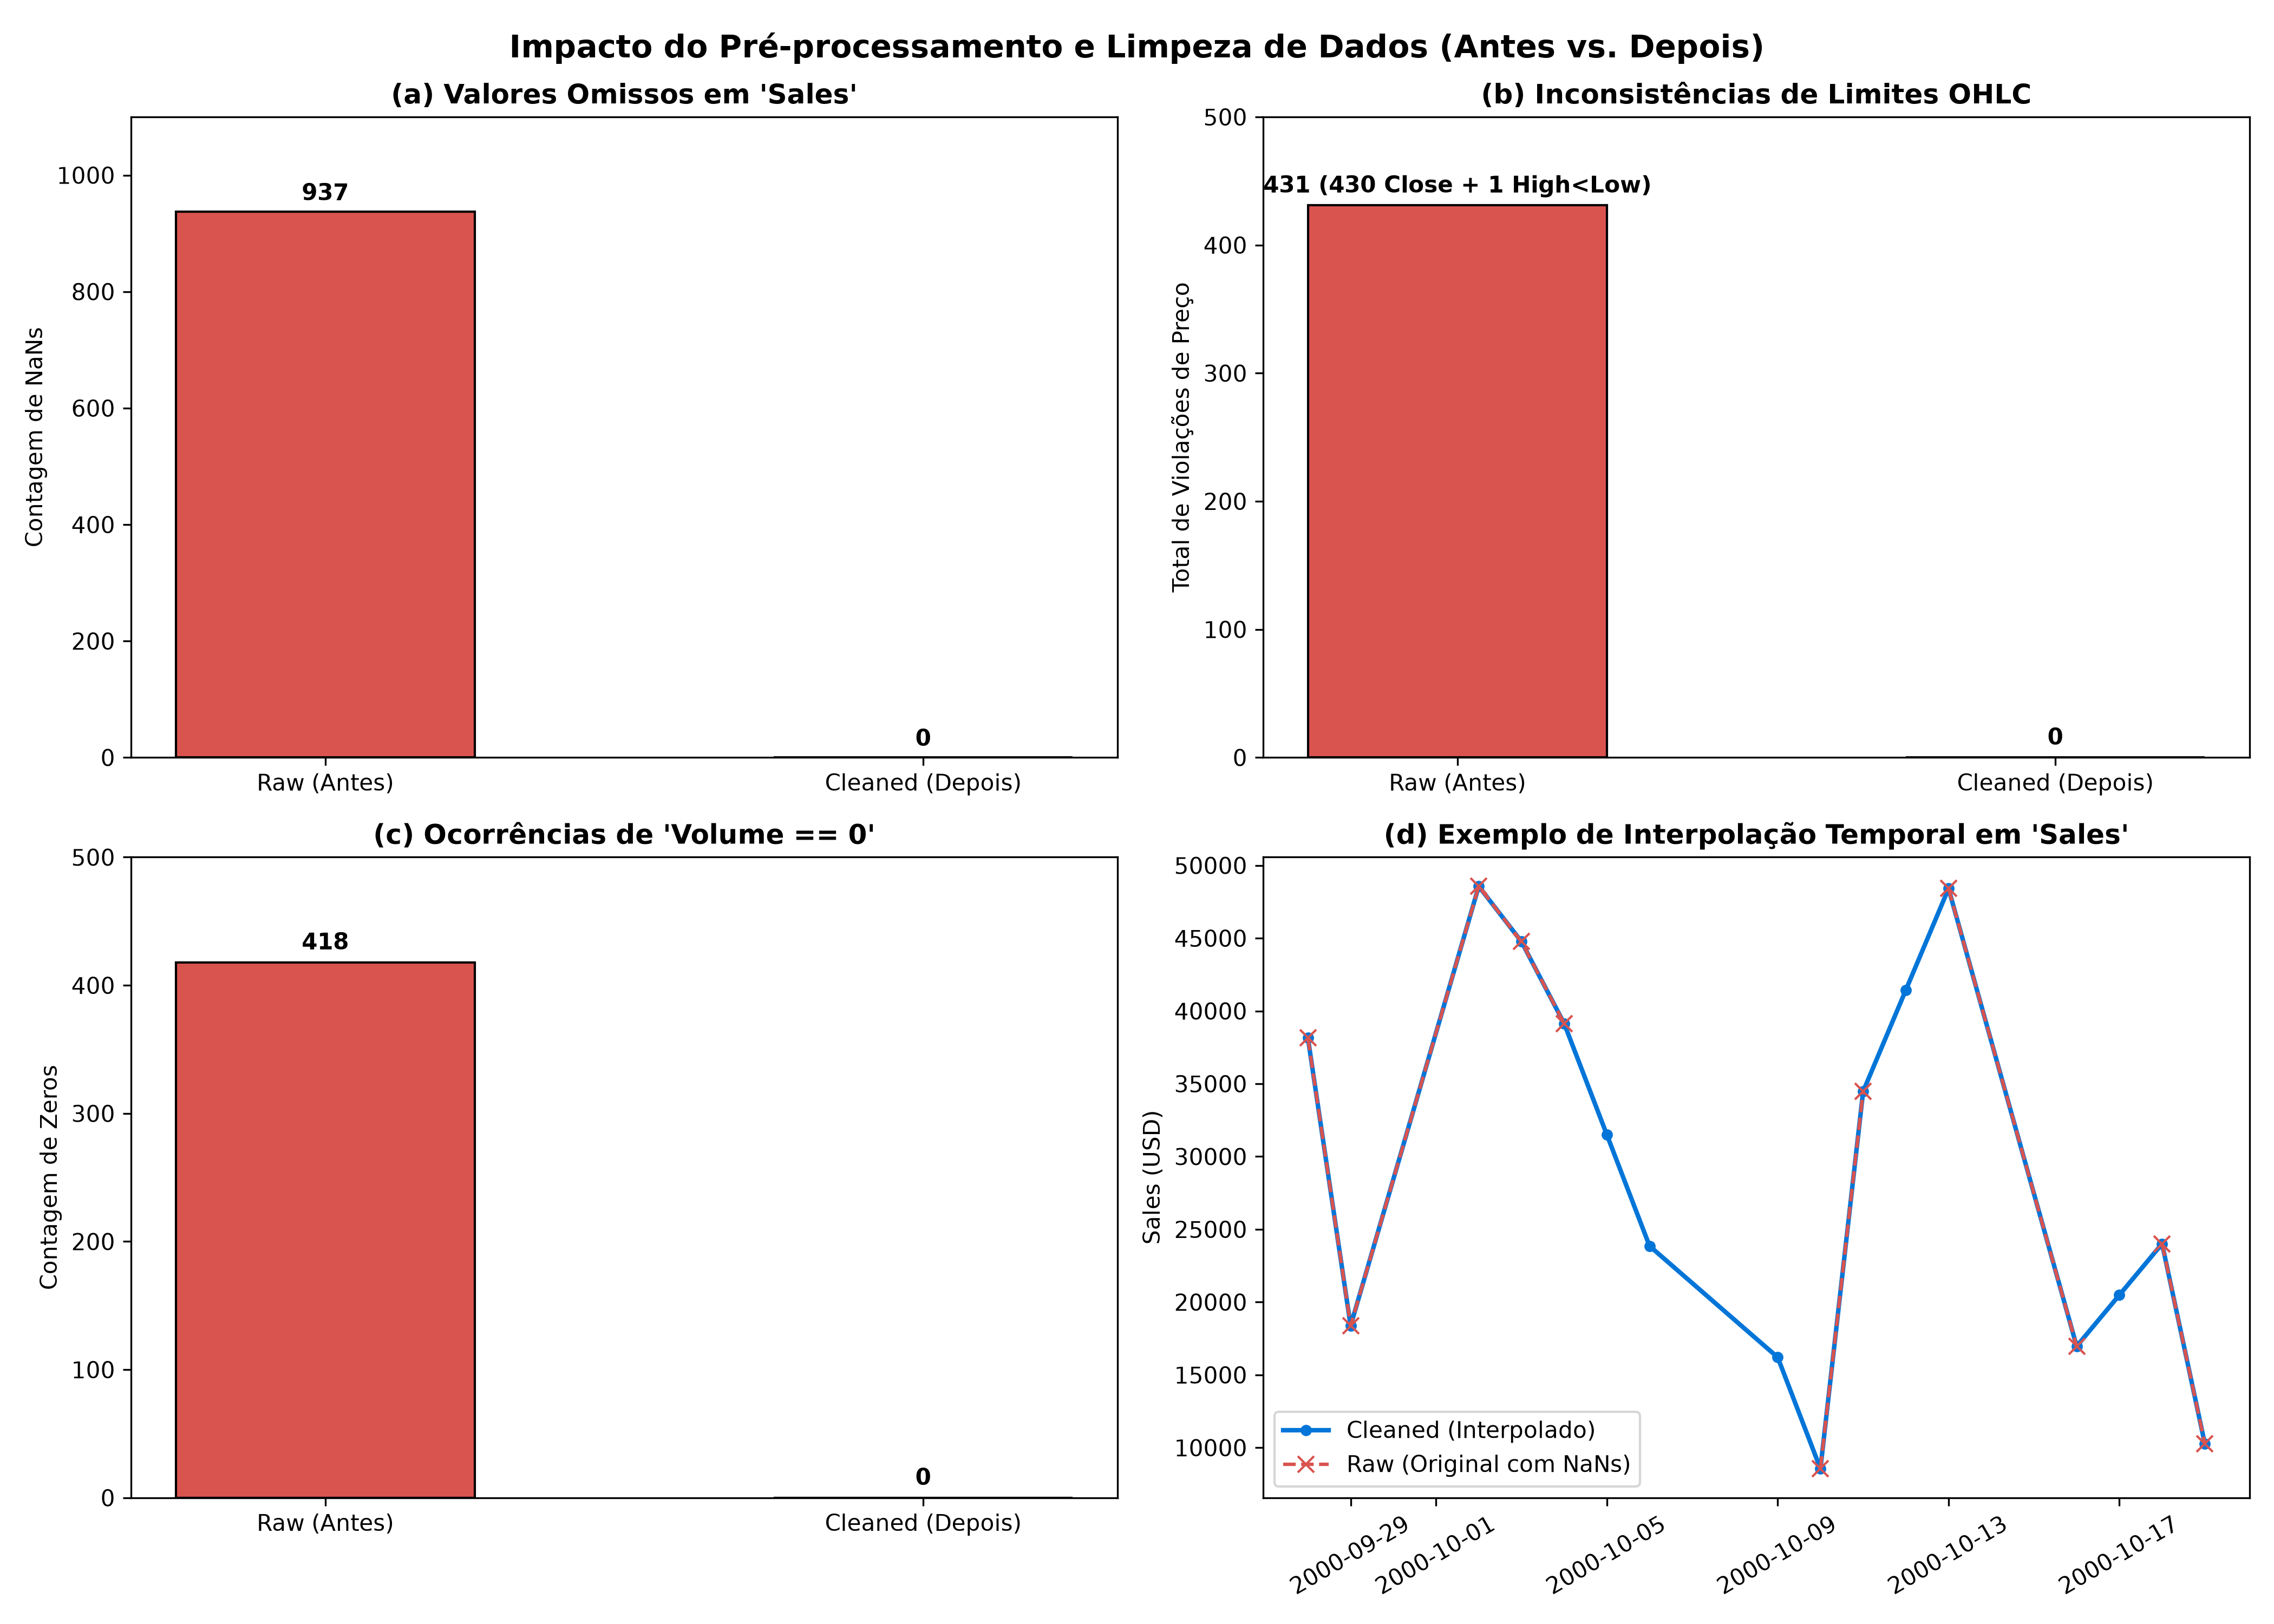
\includegraphics[width=\columnwidth]{../outputs/cleaning_effects.png}
\caption{Empirical impact of the preprocessing pipeline: (a) eradication of missing values in \texttt{Sales}, (b) elimination of OHLC price boundary violations, (c) rectification of zero-volume days, and (d) illustrative segment of continuous temporal interpolation for \texttt{Sales}.}
\label{fig:cleaning_effects}
\end{figure}

\section{Results}

\section{Discussion}

\section{Conclusion}

\begin{thebibliography}{00}
\bibitem{b1}

\end{thebibliography}

\end{document}